\documentclass[12pt]{scrbook}
\usepackage{geometry}
\usepackage{graphicx}
\usepackage{import}
\usepackage{xcolor}
\usepackage{listings}
\usepackage{caption}
\usepackage{hyperref}
\usepackage{tikz}
\usetikzlibrary{calc,positioning,shapes.geometric}

\geometry{a4paper}
\setlength{\parindent}{0pt}

\DeclareCaptionFormat{listing}{\colorbox{black!15}
  {\parbox{5cm}{#1#2#3}}}
\captionsetup[lstlisting]{format=listing,
%labelfont=white,textfont=white,
singlelinecheck=false, margin=0pt, font={bf,footnotesize}}

\newcommand{\OpenPEARL}{\textit{OpenPEARL}}

\begin{document}
\title{\OpenPEARL{} - Inter Module Checker (imc v3)}

\author{R. M\"uller}

\lstnewenvironment{XMLCode} {
    \lstset{numbers=left,
            title={XML},
            frame=tlrb,
            breaklines = true,
            belowcaptionskip=4pt
    }
}%
{}%

\lstnewenvironment{CppCode} {
    \lstset{numbers=left,
            title={C++},
            frame=tlrb,
            breaklines = true,
            belowcaptionskip=4pt
    }
}%
{}%

\lstnewenvironment{PEARLCode} {
    \lstset{numbers=left,
            title={PEARL},
            frame=tlrb,
            breaklines = true,
            belowcaptionskip=4pt
    }
}%
{}%
\pagestyle{myheadings}
\markboth {\OpenPEARL{} imc v3 \today} {\OpenPEARL{} imc v3  \today}

\date{
\today
}

\maketitle

\tableofcontents

\chapter{Introduction}
A PEARL program consists of several separatly compilable modules.
The interface between the modules is defined by SPC and DCL statements with the
attribute GLOBAL.
The GLOBAL statement has an optioal parameter for the module which defines the symbol.
In OpenPEARL, this parameter default to the actual module name. This suits for the specification
of SYSTEM part elements of the same module. 
The declaration of plattform dependent elements like INTERRUPTs, 
DATIONs and SIGNALs must be done in the SYSTEM-part.

For proper operation the types of the specified and declared elements must
fit. 
For system elements, we need a mechanism to obtain the type in an
extensible way. This is solved by the use of an interface definition as 
xml-file for each system element.

This tool checks all global definitions and specifications and checks for
\begin{itemize}
\item proper types, including the types of system elements
\item multiple declarations
\item missing declarations
\item unused declarations
\end{itemize}

\section{Structure}
As shown in \cite{mueller2016} the structure of operation of the \OpenPEARL{}
compilation system is like:
\newcommand*\circled[1]{\tikz[baseline=(char.base)]{
   \node[shape=circle,fill=white,draw,minimum size = 0.5cm, inner sep=2pt] (char) {#1};}}

\begin{figure}[bpht]

  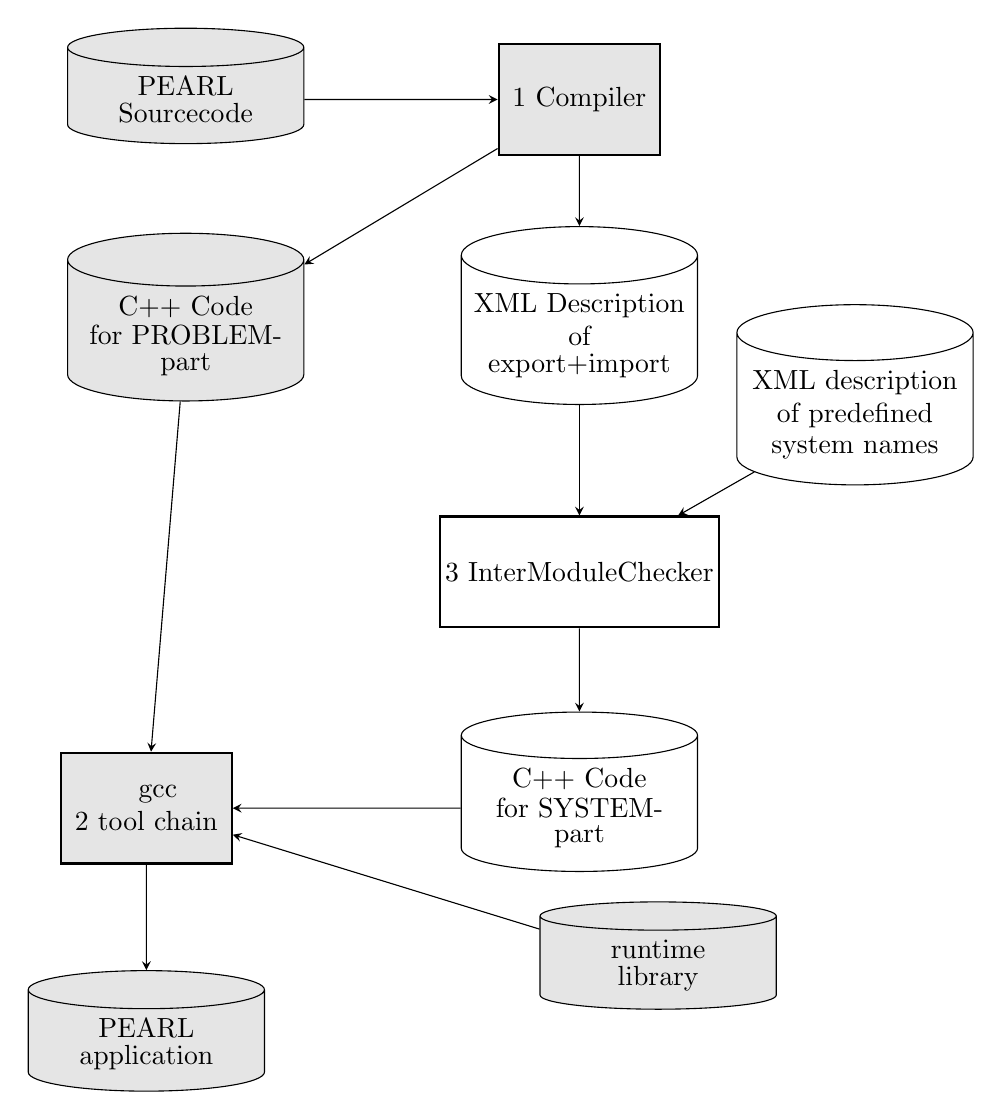
\begin{tikzpicture}[
    >=stealth,
    node distance=3.5cm,
    file/.style={
      cylinder,
      cylinder uses custom fill,
      %cylinder body fill=yellow!50,
      %cylinder end fill=yellow!50,
      shape border rotate=90,
      minimum width=3cm,
      aspect=0.25,
      draw
    },
        fileold/.style={
          cylinder,
          cylinder uses custom fill,
          cylinder body fill=gray!20,
          cylinder end fill=gray!20,
          shape border rotate=90,
          minimum width=3cm,
          aspect=0.25,
          draw
        },
    block/.style = { rectangle,
    				draw=black,
    				 thick, 
                    %fill=blue!20,
                    text centered, minimum width=5em,
                    %rounded corners,
                    inner sep = 2pt,
                    minimum height=4em },
    blockold/.style = { rectangle,
       				draw=black,
       				 thick, 
                       fill=gray!20,
                       text centered, minimum width=5em,
                       %rounded corners,
                       inner sep = 0.5em,
                       minimum height=4em }                          
  ]
    \node[fileold] (prl) at (0,10) {\shortstack{PEARL\\Sourcecode}};
    \node[blockold] (sprachumsetzer) at (5,10) {\circled{1} Compiler};
    \node[fileold,below of=prl,yshift=0.5cm] (problemcc) {\shortstack{C++ Code\\for PROBLEM-\\part}};
    \node[file,below of=sprachumsetzer,yshift=0.5cm] (modulxml) {\shortstack{XML Description
                                                            \\of \\
                                                             export+import}};
    \draw[->] (prl) -- (sprachumsetzer);
    \draw[->] (sprachumsetzer) -- (problemcc);
    \draw[->] (sprachumsetzer) -- (modulxml);

    \node[file, yshift=-1cm,right of=modulxml] (hardwarexml) {\shortstack{XML description \\of predefined\\system names}};
    \node[block, below of=modulxml,yshift=0.5cm] (imc) {\circled{3} InterModuleChecker};

    \draw [->] (modulxml) --  (imc);
    \draw [->] (hardwarexml) -- (imc);
    
    \node[file, below of=imc,yshift=0.5cm] (systemcc) {\shortstack{C++ Code\\ for SYSTEM- \\part}};
    \node[fileold, below of=systemcc, yshift=1.5cm, xshift=1cm] (runtimelib) {\shortstack{runtime\\library}};
    \node[blockold, left of=systemcc,xshift=-2cm] (gcc)
    {\circled{2}
    {\shortstack{gcc\\tool chain}}};
    \draw[->] (imc) -- (systemcc);
    \draw[->] (systemcc) -- (gcc);
    \draw[->] (runtimelib) -- (gcc);
    \draw[->] (problemcc) -- (gcc);
    
    \node[fileold, below of=gcc,yshift=0.5cm] (pearlapp) {\shortstack{PEARL\\application}};
    \draw[->] (gcc) -- (pearlapp);
  \end{tikzpicture}
\caption{Structure of the \OpenPEARL{} build system.}
\label{aufbau}
\end{figure}



The first stage compiler creates an C++-representation of the PEARL-module
together with an xml-representation of the export and import interface.

The definition of system names may be done by the user to order to supply 
additional system devices.
Each system name must be accompanied by the developer with a xml-representation
of the system element. The imc tool extracts the required information
from these xml-files and verifies a proper system configuration.

\section{Credits}
This tool  was influenced by the master thesis of 
Stephan Hertig \cite{msc_hertwig}, the semester project of
M.Bauer, T-Schaz, J.Weber, T.Welte and J.Wirth \cite{openpearlss16} and
the master thesis of M. Beyer \cite{msc_beyer}.



\chapter{Platform Specific Names}

\section{Introduction}
Each specific platform may support a different set of system names.
Thus each target platform is characterized by a separate xml-file.
These files are created during the build phase of the runtime system
for each target platform.

All possible system elements are located as unordered separate 
elements under the root tag \verb|platform|.
For the individual types of system elements, the following tags are
provided:
\begin{itemize}
\item \verb|<signal ...>| defines a system signal
\item \verb|<interrupt ...>| defines a system interupt
\item \verb|<dation ...>| defines a system dation
\item \verb|<configuration ...>| defines a configuration item
\item \verb|<connection ...>| defines a association provider, if 
   non of the above fit
\end{itemize}

These elements may have attributes 
\begin{description}
\item [name] is mandatory the system name
\item [priority] in optional the priority of instanciation. 
   The values are according the PEARL priorities. The default value is 255.
\item [private] which indicates, that this element may not be 
  refered in the system part
\end{description}

These elements may have other elements as subtree to define parameters, associations and checks.

\paragraph{Note:} The tags are interpreted by the IMC case insensitive. The XML-reader 
expects a  proper XML structure.

\section{Tags in the XML-File}
\subsection{Signal-Tag}
The signal tag contains only the attribute \verb|name| for the
system signal name.

\subsection{Interrupt-Tag}
The interrupt tag contains the attribute \verb|name| for the
system interrupt name.
Possible parameters are listed as subtree \verb|<parameters>|.

\subsection{Dation-Tag}
The dation tag contains the attribute \verb|name| for the
system dation name.
Possible parameters are listed as subtree \verb|<parameters>|.
Possible attributes are listed as subtree \verb|<attributes>|.
Possible associations to this element are
 listed as subtree \verb|<associationProvider>|.
If a system dation requires TFU in the user dation, that tag
\verb|<TFU size="80"/>| specifies the minimum record size of the 
userdation.


\subsection{Configuration-Tag}
The configuration element has the same structure as the dation tag
except the attribute \verb|name|, which has not to be present.

\subsection{autoInstanciation Attribute}
A special attribute tag is reserved for
blocking of gpio bits, which are used by system devices like i2c or 
other applications. It may be used for dation, interrupt or signal and 
needs a name-attribute for assistance.
\begin{XMLCode}
<dation name="reservedGpios" autoInstanciate="1">
  <checks>
    <check pinDoesNotCollide="RPiGPIO" bitList="0,1,2,4,6,26"/>
  </checks>
</dation>
\end{XMLCode}

Regard:
\begin{itemize}
\item autoInstanciate
  One instance of this item is instanciated automatically -- used e.g. 
  for reserved  GPIO bits
  This attribute prohibits the usage by the PEARL application in the system part
\item pinDoesNotCollide must have  the same name as used in the gpio rules in 
   e.g. RPiDigitalIn.xml
\item bitList is created from the the configuration item in \textit{menuconfig}.
The tool \texttt{convertList} is used in the \textit{Makefile} to create this list.
\end{itemize}

\subsection{Associations}
The connection between two system elements is treated by the following
elements:

\begin{itemize}
\item \verb|<needAssociation>| with the attribute 
 \verb|name| and the identifier of the expected interface. The 
  interface names are described in the runtime documentation. 
\item \verb|<associationProvider>|  with elements \verb|<associationType>|.
  Attributes for an associationType are:
  \begin{itemize}
   \item  \verb|<name>|,  which is an unique free selectable
     identifier for this kind of  association.
   \item \verb|<clients>|  if given it is the number of allowed
      clients for this connection provider. If not given, there is no
      limits of allowed clients.
   \end{itemize} 
\end{itemize}

\paragraph{Note:} An association may have another association.
 
\section{Parameters}
Only parameters of system elements of types bit, fixed and char are supported.
The actual value may be restricted to definite values and ranges.

Each parameter tag must have an attribute name, which is used as nickname 
for checks of allowed values, combinational useage and error messages.
The name must consist only of characters. Camelcase notation should be used.

Tags are defined for each of them:
\begin{itemize}
\item \verb|BIT| with the attribute \verb|length|, which specifies the 
   allowed length of an actual parameter. \verb|<BIT length="8">...</BIT>|
   specifies a BIT(8) parameter. Shorter actual parameters are extended --- 
   longer parameters induce an error message.
\item \verb|FIXED| with the attribute \verb|length|, which specifies the 
   allowed length of an actual parameter. \verb|<FIXED length="15">...</FIXED>|
   specifies a FIXED(15) parameter. Shorter actual parameters are extended --- 
   longer parameters induce an error message.
\item \verb|CHAR| with the attribute \verb|length|, which specifies the 
   allowed length of an actual parameter. \verb|<CHAR length="15">...</CHAR>|
   specifies a CHAR(15) parameter. Shorter actual parameters are allowed --- 
   longer parameters induce an error message.
\end{itemize}

\subsection{Expressions and Checks for and upon Parameter Values}
Parameters are checked by the IMC against some rules. Each parameter
must provide the attribute name, which  consists only of characters. 

In rules these parameters may be used in expressions.
To access a parameter name, an '\$' must be used as prefix.
Expressions are supported for integer results. The expression 
evaluator treats only the type integer.
Nested expressions must be placed in square brackets:
e.g. \verb|anyText[$start+3]anyOtherText|.


Supported rules:

\begin{tabular}{|l|c|p{8cm}|}
\hline
rule & type & description \\
\hline
VALUES & BIT,FIXED, CHAR &
   a comma separated list of allowed values
   is given. Other values produce an error message. 
No nicknames or expressions are allowed.\\
\hline
ConsistsOf & CHAR &
a comma separated list of allowed values is given. 
The actual parameter must consist of only one or more of these
elements.
No name references or expressions are allowed.\\
\hline
NotEmpty & CHAR & 
   at least one character is required \\   
\hline
FIXEDRANGE & FIXED &
   two comma separated integers or expressions with nicknames
 limits the allowed range
   of actual values --- borders included \\ 
\hline
FIXEDGT & FIXED &
   one integer or expression with nicknames
 limits the allowed range at the low side
   of actual value --- border NOT included \\ 
\hline
\end{tabular}

\paragraph{Note:} If other checks are needed, they must become implemented in 
\verb|checks/CheckSyspart.java|.

\section{Consistency Checks between all System Part Elements}
Different system part elements may violate some hardware restictions.
Thus an GPIO pin may only be used as input or output, or on microcontrollers
an GPIO may only be used as digital io or as alternate function like UART comminication.

The XML-tag \verb|<check...>| defines checks, which are executed
over all defines system elements in all modules.

\subsection{Types of Checks}
%Depending on the concrete system element 
%\begin{itemize}
%\item only one instance is allowed, or
%\item multiple instances are allowed as long as some parameters differ, or
%\item e.g. on I2C devices, the I2C address must be unique / not unique on 
%a dedicated i2c bus.  
%\item GPIO bits a microcontrollers and I2C port expander may only used once, or
%\item a multiplexer channel of a dedicated device may only be used once, or
%\item ...
%\end{itemize}

If such a restriction applies  to a system element some rules must be supplied 
in the platform definition.

To some restrictions must have access to instance parameters and instance association.
Instance parameters are accessed via \$ and their name.

\subsubsection{Number of Instances}
\begin{description}
% obsolete: may be realized via oncePerSet set="StdOut"
%\item[instances="1"] only one instance of the platform system element
%   is allowed (like  Log, Console or StdIn)
\item[instances="oncePerSet" set="..."] defines that only one instance with a 
  specified set of parameters are allowed. To define a set we have access to 
  all parameter names and in case of associations the complete association list.
  The attribute set defines a string identifying the set selector. 
  \newline
  Example: Several I2C busses in a system need different system interfaces

  \begin{PEARLCode}
  SYSTEM;
     ! this sample is ok, different unix interfaces
     i2cbus0 : I2CBus('/dev/i2c-0');
     i2cbus1 : I2CBus('/dev/i2c-1');
  \end{PEARLCode}

  Check definition in platform:
  
  \begin{verbatim}
  <connection name="I2CBus" ...>
    <parameters>
       <CHAR name ="deviceName" length="32767">
          <NotEmpty />
       </CHAR>
    </parameters>
    ...
    <check instances="oncePerSet" set="I2CBus($deviceName)"/>
  \end{verbatim}

  The imc maintains a list of all instances of the platform element.
  Multiple instances with different \textit{deviceNames} are ok.
  Multiple instances with the same \textit{deviceName} result is
  error messages.

  The example enshures that there is only one instanciation of 
  one I2C interface. 
\end{description}

\subsubsection{Pin Usage does not collide}
I/o bits are available on GPIOs of microcontrollers and on port expanders.
The adressing of bits are traditionally done by the parameters
\textit{most significant bit numer} and
\textit{number of bits}. These two parameter define the i/o bits of the 
digital i/o component.

Especially on microcontrollers other system devices use GPIO bits, which 
are only available for ether digital i/o or special function.

\begin{description}
\item[pinDoesNotCollide="..."]

Example: PCF8574-port expander on the I2CBus('/dev/i2c-0')
  \begin{PEARLCode}
  i2cBus: I2CBus('/dev/i2c-0');
  !                             76543210
  ! conflict bitsIn3 use bits     xxx
  !          bitsOut4            xxx
  ! bits 5 and 4 are used duplicate 
  bitsIn3:  PCF8574In('44'B4, 5, 3) --- i2cBus;
  bitsOut4: PCF8574In('44'B4, 6, 3) --- i2cBus;
  \end{PEARLCode}

  Check definition in platform:
  \begin{verbatim}
  <check pinDoesNotCollide="PCF8574($i2cAddr)" start="$start" width="$width"/>  
  \end{verbatim}
  \begin{itemize}
  \item The complete chain of association providers is added automatically
  the pinDoesNotCollide selector. 
  The provider evaluates to \verb|I2CBus('/dev/i2c-0')| even
  the provider is specified by an user supplied name.

  \item \verb|PCF8574| is a fixed text. The same text will be used in the PCF8574In
  device prohibiting the usage of a bit simultaneously as input and output.

  \item \verb|$i2cAddr| evaluates to \verb|'44B4'|

  \item \verb|$start| evaluates to  5 at bitsIn3 

  \item \verb|$width| evaluates to 3

  \end{itemize}

The imc creates a list of used pins on the given instance. 
Note that the numbers are not identical to the pin numbers of
the i/o chip. 
In case a pin is already allocated by another instance an error
message will be emitted.

Note that \$width is optional and defaults to 1.

Note that an optional attribute \verb|errorText=".."| exists, which allows 
to modify the error message. This is useful to create more compreghensive 
error messages if the check is applied on e.g. adc multiplexer channels:
 \texttt{errorText="adc channel"}, which replaces the default text "pin".

\item[i2cAdrDoesNotCollide="..."] adresses the problem that 
  different i2c devices must have different adresses on a dedicated
  i2c bus. E.g. in case of port expander we may have multiple
  instances of the same i2c device on the same bus.

  Example: 

  \begin{PEARLCode}
  SYSTEM;
    ! all ok; bits3 and bits2 use diffenent pins they use
    ! the same i2c device PCF8574.
    i2cbus: I2CBus('dev/i2c-0');
    bits3: PCF8574In('44'B4, 5, 3) --- i2cbus;
    bits2: PCF8574In('44'B4, 7, 2) --- i2cbus;
    temp1: LM75('48') --- i2cbus;
    temp1: LM75('49') --- i2cbus;
  \end{PEARLCode}

  Checks definition in platform:

  \begin{verbatim}
  <dation name="PCF8574In" ..
      <parameters>
      ...
     </parameters>
     <needAssociation name="I2CBusProvider"/>
     <checks>
     <check i2cAdrDoesNotCollide="PCF8574" sharable="$iicAdr" />
     <check pinDoesNotCollide="..." />
     </checks>

   ...
  <dation name="PCF8574Out" ..
      <parameters>
      ...
     </parameters>
     <needAssociation name="I2CBusProvider"/>
     <checks>
        <check i2cAdrDoesNotCollide="PCF8574" sharable="$iicAdr" />
        <check pinDoesNotCollide="..." />
     </checks>
   ...

   <dation name="LM75" ...
     <system name="LM75">
     ...
     <needAssociation name="I2CBusProvider"/>
     ...
     <checks>
     <check i2cAdrDoesNotCollide="LM75" nonSharable="$iicAdr" />
     </checks>

        <connection name="I2CBus">
         <parameters>
            <CHAR name="deviceName" length="32767">
               <NotEmpty />
            </CHAR>
         </parameters>
         <associationProvider>
            <associationType name="I2CBusProvider" />
         </associationProvider>
         <checks>
           <check instances ="oncePerSet" set="I2CBus($deviceName)"/>
         </checks>
      </connection>

  \end{verbatim}

  \paragraph{Note:} The name of the parameter \verb|iicAdr| must not be written
  as \verb|i2cAdr| since a parameter name consists only of letters.

  The imc maintains a list of all I2CBusProvider elements.
  For each I2CBusProvider the imc maintains a list of all  i2c components
  on this i2c bus.
  If the same  adress is used by different devices we have an error condition.
  If the same  adress is used by the same device we have an error condition if
  the device does not support multiple usage like a port expander.
\end{description}

If more checks are required, they can be added in \texttt{imc/checks}. 

\subsection{needItem}

A needItem tag forces to instanciate one instance of the given system element.
This is needed by interrupts at the raspberry pi gpio lines. The interrupts are
specified in separate syystem part definitions. 
The treatment of these interrupts requires a single thread to receive the 
interrupt events.

 
\section{Platform File}
Each system part elements is represented by a driver in the OpenPEARL 
source tree and an XML-snipplet. These snipplets are
concatenated to the Platform Definition File during the build  process.

Example:
\begin{XMLCode}
<?xml version="1.0" encoding="UTF-8"?>
<platform file="testPlatform.xml">
      <signal name="FixedRangeSignal"/>
      <signal name="FixedDivideByZeroSignal"/>
      <signal name="FloatIsNaNSignal"/>

      <interrupt name="UnixSignal">
         <parameters>
            <FIXED name="signalNumber" length="31">
               <VALUES>1,2,3,15,16,17</VALUES>
            </FIXED>
         </parameters>
      </interrupt>

      <dation name="Disc">
         <parameters>
            <CHAR name="dir" length="32767"/>	<!-- beliebiger String -->
            <FIXED name="nbrOfFiles" length="31">
               <FIXEDRANGE>1,9999</FIXEDRANGE>
            </FIXED>
         </parameters>
         <attributes>FORWARD, DIRECT, IN, OUT, INOUT, SYSTEM</attributes>
         <data>ALL</data>
         <associationProvider>
            <associationType name="NamedAlphicOutProvider" />
         </associationProvider>
      </dation>

      <dation name="StdIn">
         <parameters>
         </parameters>
         <attributes>
            FORWARD, IN	, SYSTEM
         </attributes>
         <DATA>ALPHIC</DATA>
         <checks>
           <check instances="1"/>
         </checks>
      </dation>

      <dation name="StdOut">
         <parameters>
         </parameters>
	 <attributes>
            FORWARD, OUT, SYSTEM
         </attributes>
         <data>ALPHIC</data>
         <associationProvider>
            <associationType name="AlphicOutProvider" />
         </associationProvider>
         <checks>
           <check instances ="1"/>
         </checks>
      </dation>

      <connection name="I2CBus">
         <parameters>
            <CHAR name="deviceName" length="32767">
               <NotEmpty />
            </CHAR>
         </parameters>
         <associationProvider>
            <associationType name="I2CBusProvider" />
         </associationProvider>
         <checks>
           <check instances ="oncePerSet" set="I2CBus($deviceName)"/>
         </checks>
      </connection>

      <dation name="LM75">
         <parameters>
            <BIT name="iicAdr" length="8">
               <VALUES>'20'B4,'48'B4, '49'B4, '4A'B4, '4B'B4,
                       '4C'B4, '4D'B4 , '4E'B4, '4F'B4</VALUES>
            </BIT>
         </parameters>
	 <attributes>
            BASIC, SYSTEM, IN
         </attributes>
         <data>FIXED(15)</data>
         <needAssociation name="I2CBusProvider"/>
         <checks>
           <check i2cAdrDoesNotCollide="LM75"
                   nonShareable="$iicAdr"/>
         </checks>
      </dation>

      <dation name="PCF8574In">
         <parameters>
            <BIT name="iicAdr" length="8">
               <VALUES>'20'B4, '21'B4, '22'B4, '23'B4,
                       '24'B4, '25'B4 , '26'B4, '27'B4,
                       '38'B4, '39'B4 , '3A'B4, '3B'B4,
                       '3C'B4, '3D'B4 , '3E'B4, '3F'B4
               </VALUES>
            </BIT>
            <FIXED length="7" name="start">
               <FIXEDRANGE>0,7</FIXEDRANGE>
            </FIXED>
            <FIXED length="7" name="width">
               <FIXEDRANGE>1,[$start+1]</FIXEDRANGE>
            </FIXED>
         </parameters>
	 <attributes>
            BASIC, SYSTEM, IN
         </attributes>
         <data>BIT($width)</data>
         <needAssociation name="I2CBusProvider"/>
         <checks>
           <check pinDoesNotCollide="PCF8574xx(I2cAdr=$iicAdr)" 
		start="$start" width= "$width" />
           <check i2cAdrDoesNotCollide="PCF8574"
                   shareable="$iicAdr"/>
         </checks>
      </dation>

      <dation name="PCF8574Out">
         <parameters>
            <BIT name="iicAdr" length="8">
               <VALUES>'20'B4, '21'B4, '22'B4, '23'B4,
                       '24'B4, '25'B4 , '26'B4, '27'B4,
                       '38'B4, '39'B4 , '3A'B4, '3B'B4,
                       '3C'B4, '3D'B4 , '3E'B4, '3F'B4
               </VALUES>
            </BIT>
            <FIXED length="7" name="start">
               <FIXEDRANGE>0,7</FIXEDRANGE>
            </FIXED>
            <FIXED length="7" name="width">
               <FIXEDRANGE>1,[$start+1]</FIXEDRANGE>
            </FIXED>
         </parameters>
	 <attributes>
            BASIC, SYSTEM, OUT
         </attributes>
         <data>BIT($width)</data>
         <needAssociation name="I2CBusProvider"/>
         <checks>
           <check pinDoesNotCollide="PCF8574xx(I2cAdr=$iicAdr)" 
		start="$start" width= "$width"/>
           <check i2cAdrDoesNotCollide="PCF8574"
                   shareable="$iicAdr"/>
         </checks>
      </dation>

  <configuration name="Log">
    <parameters>
      <CHAR name="loglevel" length="4">
         <NotEmpty/>
      </CHAR>
    </parameters>
    <needAssociation name="AlphicOutProvider"/>
    <checks>
       <check instances ="1"/>
    </checks>
  </configuration>

   <connection name="LogFile">
      <parameters>
         <CHAR name="fileName" length="32767">
            <NotEmpty/>
         </CHAR>
      </parameters>
      <associationProvider>
         <associationType name="AlphicOutProvider"/>
      </associationProvider>
      <needAssociation name="NamedAlphicOutProvider"/>
   </connection>

   <dation name="RPiDigitalIn">
      <parameters>
         <FIXED name="start" length="31">
             <FIXEDRANGE>0,27</FIXEDRANGE>
         </FIXED>
         <FIXED length="31" name="width"> <FIXEDGT>0</FIXEDGT></FIXED>
         <CHAR name="pullUpDown" length="1"><VALUES>'u','d','n'</VALUES></CHAR>
      </parameters>
      <attributes> IN, SYSTEM, BASIC</attributes>
         <checks>
           <check pinDoesNotCollide="RPiGPIO" 
		start="$start" width= "$width"/>
           </checks>
      <data>BIT($width)</data>
   </dation>

   <dation name="RPiDigitalOut">
      <parameters>
         <FIXED name="start" length="31">
             <FIXEDRANGE>0,27</FIXEDRANGE>
         </FIXED>
         <FIXED length="31" name="width"> <FIXEDGT>0</FIXEDGT></FIXED>
      </parameters>
         <checks>
           <check pinDoesNotCollide="RPiGPIO" 
		start="$start" width= "$width"/>
           </checks>
      <attributes> OUT, SYSTEM, BASIC</attributes>
      <data>BIT($width)</data>
   </dation>

   <configuration name="reservedGpios" autoInstanciate="1">
     <checks>
      <check pinDoesNotCollide="RPiGPIO" bitList="0,1,2,4,5,6,7"/>
     </checks>
   </configuration>

</platform>
\end{XMLCode}

\chapter{Structure of Module Import and Export Definition}

The compiler creates an xml-file per PEARL-module containing the
\begin{itemize}
\item system part information
\item problem part specifications and declarations
\end{itemize}

This chapter describes the interface to the compiler.

\section{XML-Document Structure}
The compiler has no knowledges about the nature of a system name.
Thus the system part is translated as it is --- only syntactical errors
are recognized. 
The document has the root tag \verb|<module>|, which hat the attribute
\verb|file| with the value source file name.  
All system elements are in the xml-subtree \verb|<system>|.
All problem part elements with attribute GLOBAL are located
in the xml-subtree \verb|problem|.
Locally defined  DATIONs are also exported in the xml-subree \verb|problem| 
for compatibility tests with the system dation.

\begin{XMLCode}
<?xml version="1.0" encoding="UTF-8" ?>
<module file="demo.prl">
<system>
   <username .... >
   ....
   </username>
   <configuration .... >
   ....
   </configuration>
</system>
<problem>
  <spc .../>
  <dcl .../>
  ...
</problem>
</module>
\end{XMLCode}

\section{System Part Elements}
\subsection{User Names \texttt{<username>}}
If a system element defines a user name the \verb|<username>| tag is 
used. Each user name is accompanied by an system name with the tag 
\verb|<sysname>|, which may have parameters.
The sysname-tag may contain a list of associations, thus there may by a tree
of \verb|<association>| tags.
The user name tag contains the attribute \verb|line| with the value of the 
source code line number.

\subsection{System Name \texttt{<sysname>}}
The system name tag contains the attribute \verb|name| containing the 
name of the system element.

\subsection{Parameters \texttt{<parameters>}}
\label{sec_parameters}
The parameters are located in the \verb|<parameters>|-subtree.
The imc tool supports constants of type FIXED, CHAR and BIT.
The compiler detects  the type of the parameter
from the literal and passes the literal as content to the corresponding
\verb|<FIXED>|-, \verb|<CHAR>|- or \verb|<BIT>|-tag.

\subsection{Associations \texttt{<association>}}
An association may be ether a system name (with parameters) or a user name.
The  \verb|<association>|-tag contains the attribute \verb|name| with the 
given name as value. If parameters are specified for the association,
they are passed as \verb|<parameters>|-subtree in the same way as decribed 
in section \ref{sec_parameters}.

There is no check in the compilation phase done,
whether a name is a system name
or a user supplied name.

As defined in the grammar of OpenPEARL an association may lead to a 
connection provider which has another association.
Example:
\begin{PEARLCode}
SYSTEM;
  Log('EW') --- LogFile('pearl_log.txt') --- DISC('./',1);
\end{PEARLCode}


\subsection{Configuration Item}
Configuration elements in the system part are located in the
\verb|<configuration>|-element. 
The only difference to the \verb|<username>|-tag is the absence of the 
\verb|name|-attribute. Parameters and associations apply identical.

\subsection{Example for System Part Elements and their Specifications}
The following example contain two declaractions of the same I2C interface.
It depends on the platform definition wether this is allowed or not. For I2CBus 
interfaces this would be not allowed on the same device-node.

\begin{PEARLCode}
MODULE(demo);

SYSTEM;
lm75: LM75('48'B4) --- I2CBus('/dev/i2c-0');

lm75: LM75('48'B4) --- i2cbus1;
i2cbus1: I2CBus('/dev/i2c-1');

sig1: FixedRangeSignal;
int1: UnixSignal(15);

disc: Disc('/tmp/folder1', 10);

stdOut: StdOut;

Log('EW') --- StdOut;

PROBLEM,
SPC sig1 SIGNAL GLOBAL;
SPC int1 INTERRUPT GLOBAL;
SPC disc DATION OUT DIRECT SYSTEM ALL GLOBAL;
SPC stdOut DATION OUT SYSTEM ALPHIC GLOBAL;
SPC lm75 DATION IN SYSTEM FIXED(15) GLOBAL;

MODEND;
\end{PEARLCode}

\begin{XMLCode}
<?xml version="1.0" encoding="UTF-8" ?>
<module file="demo.prl">
<system>
   <username name="lm75" line="4">
      <sysname name="LM75">
      <parameters>
         <BIT>'48'B4</BIT>
      </parameters>
      <association name="I2CBus">
         <parameters>
            <CHAR>'/dev/i2c-0'</CHAR>
         </parameters>
      </association>
   </sysname>
</username>

<username name="lm75a" line="6">
   <sysname name="LM75">
      <parameters>
         <BIT>'49'B4</BIT>
      </parameters>
      <association name="i2cbus1">
      </association>
   </sysname>
</username>

<username name="i2cbus1" line="7">
   <sysname name="I2CBus">
      <parameters>
         <CHAR>'/dev/i2c-1'</CHAR>
      </parameters>
   </sysname>
</username>

<username name="sig1" line="9">
   <sysname name="FixedRangeSignal"/>
</username>

<username name="int1" line="10">
   <sysname name="UnixSignal">
      <parameters>
         <FIXED>15</FIXED>
      </parameters>
   </sysname>
</username>

<username name="disc" line="12">
   <sysname name="Disc">
      <parameters>
         <CHAR>'/tmp/folder1'</CHAR>
         <FIXED>10</FIXED>
      </parameters>
   </sysname>
</username>

<username name="stdOut" line="14">
   <sysname name="StdOut">
   </sysname>
</username> 

<configuration line="16">
   <sysname name="Log">
      <parameters>
         <CHAR>'EW'</CHAR>
      </parameters>
      <association name="StdOut">
      </association>
   </sysname>
</configuration>
</system>
<problem>
<spc type="signal" name="sig1" line="19"/>
<spc type="interrupt" name="int1" line="20" />
<spc type="dation" name="disc" line="21">
   <attributes> OUT,SYSTEM, DIRECT </attributes>
   <data>ALL</data>
</spc>
<spc type="dation" name="stdOut" line="22">
      <attributes> OUT, SYSTEM </attributes>
      <data>ALPHIC</data>
</spc>
<spc type="dation" name="lm75" line="23">
      <attributes> IN, SYSTEM </attributes>
      <data>FIXED(15)</data>
</spc>
</problem>
</module>
\end{XMLCode}

\section{Problem Part Elements}
\subsection{Specification of System Part Elements}
The PEARL source code defined the type of a system name to be ether a DATION, 
INTERRUPT or SIGNAL. According detected type, the compiler 
adds a xml-tag \verb|<spc>|-tag with attributes \verb|type| anf \verb|line|
containing the value \verb|"DATION"|, \verb|"INTERRUPT"| or \verb|"SIGNAL"|,
 respectively.

While interrupts and signals have no parameters, dations need more
specifications. The attributes are stores as comma separated list in the
\verb|<attributes>|-subelement, the transmission data is given as value
of the <data>-tag. For details aboutencoding of the type information
see chapter \ref{encoding}. 

\subsection{Declaration of Problem Part Elements}

Additional type information for the \verb|type| attribute are introduced.
Simple types are donated by their PEARL type with length or precision.
Array are denoted with their virtual dimention list prepended separated by
one space character.
REF of any kind are denoted with  \texttt{REF} pnd space prepended the the
type.

Structs are denoted by their encoding rules of
structures and structure elements  as described in \cite{runtime}.

Dations contains an attribute- and data-tag like in the system part notation.

\subsection{Specification of Problem Part Elements}
The specification of global  elements in the problem part are described 
in the same as their declaration.

\subsection{Example for Specification and Declarations in Problem Part}

\begin{PEARLCode}
PROBLEM;
   DCL x FIXED(7) GLOBAL;
   SPC y FIXED(17) GLOBAL;
   DCL d12 DATION OUT STRUCT [a FIXED(7), b FLOAT(53)]
     DIM(10,20)  GLOBAL CREATED(aSystemDation);
   DCL s1 SEMA PRESET(10) GLOBAL;
\end{PEARLCode}

\begin{XMLCode}
...
<problem>
  <dcl type="FIXED(7)" name="x" line=".."/>
  <spc type="FIXED(17)" name="y" line=".."/>
  <dcl type="dation" name="d12" line="10">
    <attributes>OUT DIM(10,20)</attributes>
    <data>S5A7B57</data>
  </dcl>
  <dcl type="SEMA" name="s1" line="..."/>
</problem>
\end{XMLCode}


\subsection{Encoding of Transfer Data Types and STRUCTs}
\label{encoding}
The primitive data types and their length are encoded 
by their PEARL notation.  E.g.\verb|FIXED(7)|. The encoding rules
for struct and arrays are expected as described in \cite{runtime}. 

Special values are ALL and ALPHIC.

\begin{description}
\item[ALL] fits to all data types
\item[ALPHIC] in problem part fits to ALPHIC, CHAR and ALL in system devices
\end{description}

This mapping is also used for problem part global elements, except for dations,
which need more information to be checked.

\subsection{TFU}
The treatment of \texttt{TFU} differs, whether the system dation
requires \texttt{TFU} or not.

If the system dation requires \texttt{TFU}  the user dations created
 upon this system dation must use TFU.
The specification of a dation does not contain any information about TFU.

Example:

\begin{PEARLCode}
SYSTEM;
  con: Console;
PROBLEM;
  SPC con     DATION INOUT ALPHIC SYSTEM;
  DCL console DATION INOUT ALPHIC DIM(*,80) TFU FORWARD CREATED(con);
  DCL consol2 DATION INOUT ALPHIC DIM(*,90) TFU FORWARD CREATED(con);
  DCL noTFU   DATION INOUT ALPHIC DIM(*,80)     FORWARD CREATED(con);
\end{PEARLCode}

The name \texttt{noTFU} should cause an error message,
since the system dation \texttt{Console} requires \texttt{TFU}.

The compiler  has no information about the capabilities and details
of thesystem part elements.

To check the necessity of \texttt{TFU} and requested sizes the compiler 
exports all relevant information for the checks about \texttt{TFU}
In addition to the declaracti0on and specification of the element \texttt{con}
a separate section is exported like:

\begin{XMLCode}
 <problem>
  ...
  <tfuusage>
    <userdation name="console" lineno="23", col="7">
       <systemdation name="con"/>
       <usedTFU size="80"/>
    </userdation>
    <userdation name="console2" lineno="24", col="7">
       <systemdation name="con"/>
       <usedTFU size="90"/>
    </userdation>
    <userdation name="noTFU" lineno="25", col="7">
       <systemdation name="con"/>
    </userdation>
  </tfuusage>
\end{XMLCode}

The compiler can calculate the record size for typeOfTransmission ALL,ALPHIC or simpleType. For typeStructure - the compiler does not known the allignment
restrictions from the target depending g++-compilation.
If the type of transmission is a STRUCT - the size will be set to 0
and the check must be done at system start,
when the userdation becomes instanciated.

With this information the imc may check
\begin{itemize}
\item if the record size  of \texttt{console} fits with the requirements of 
    \texttt{con}
\item if the userdation uses \texttt{TFU} at all
\end{itemize} 

Application specific error messages can becom procuded, like:

\lstset{breaklines=true}
\begin{lstlisting}
demo.prl:24:7: error: TFU record of dation 'console2' exeeeds limit of 'Console'
demo.prl:25:7: error: dation 'noTFU' must use TFU, which is required by 'Console'
\end{lstlisting}


\section{Multi-Module Support}
The imc supports the operation modes \verb|-std=PEARL90| and \verb|-std=OpenPEARL|.

\subsection{Standard PEARL90}
In this standard only one system part is allowed and the module name is only
for documentation use.
The compiler must set the for \verb|GLOBAL| elements the value to the given name or to the empty string.

\subsection{Standard OpenPEARL}
In this standard multiple system parts are allowed.
The module name is required and defines the namespace of the objects defined in this module.
The compiler must set the for defined \verb|GLOBAL| elements the value the module name.

\subsection{Tests concerning Multi-Module}
The compiler sets the selected standard in the module tag. 
The IMC checks this element.

\chapter{Usage}

\section{Invocation}
The inter module checker is invoked with
\begin{verbatim}
imc -b <target> -o <output> pearlModules...
\end{verbatim}

The list of pearl modules is passed without extension. Pathnames are 
possible.

\section{Options}
\begin{description}
\item[-b] The option -b is  recommended. The given parameter defines the
platform definition XML file, which is expected ether in the current 
working directory (first)
or in installation directory of OpenPEARL.
\item [-o] defaults to system.cc in the current working directory. This is
  the name of the source file for the system part.
\item[-std=OpenPEARL] is default. Multiple system parts are allowed and the 
    module name defines the namespace.
\item[-std=PEARL90] allows only one system part. The module name is only used 
  for documentation. The C++ code goes into the namespace \texttt{pearlApp}.
\item[-I ] defines the installation path of the platform definition files
\item[--verbose] enables more messages 
\item[--help] prints a help message with all supported options.
\end{description}





\chapter{Documentation}

The documentation of the implementation is done in Javadoc. Please refer
the Javadoc output.



\begin{thebibliography}{99}
\bibitem{mueller2016}  
   M.Schaible, R. M\"uller; Konsistenzpr\"ufungen in OpenPEARL,
   In W.A. Halang, H. Unger (Hrsg.): Informatik aktuell --- 
   Internet der Dinge und Echtzeit, Springer Verlag, 2016

\bibitem{msc_hertwig}
    Stephan Hertwig: SmallPEARL ---
    Treiber f\"ur die Peripherieinfrastruktur des Raspberry,
    Masterthesis FernUNI Hagen, Sommerseemster 2015
 
\bibitem{openpearlss16}
    M.Bauer, T.Schaz, J.Weber, T. Welte, J. Wirth: OpenPEARL,
    Projektarbeit im Studiengang AIB/CNB der HS Furtwangen, Sommersemester 2016

\bibitem{runtime}
   R. M\"uller: OpenPEARL - Runtime System, Project Document

\bibitem{msc_beyer}
   M. Beyer: ????,
   Masterthesis HS Furtwangen, Sommersemester 2018

\end{thebibliography}
~                          


\end{document}
